\documentclass[11pt,a4paper]{article}

\usepackage[utf8]{inputenc}
\usepackage[T1]{fontenc}
\usepackage[spanish]{babel}
\usepackage{amsmath, amssymb, amsthm}
\usepackage{booktabs}
\usepackage{graphicx}
\usepackage{hyperref}
\usepackage{xcolor}
\usepackage{algorithm}
\usepackage{algpseudocode}
\usepackage{multirow}
\usepackage{geometry}
\usepackage{natbib}
\usepackage{caption}
\usepackage{subcaption}
\usepackage{enumitem}

\geometry{margin=1in}

\hypersetup{
    colorlinks=true,
    linkcolor=blue!60!black,
    citecolor=blue!60!black,
    urlcolor=blue!60!black
}

\newtheorem{definition}{Definición}
\newtheorem{proposition}{Proposición}

\title{
    \vspace{-1cm}
    \textbf{Selección de Métricas para la Evaluación Objetiva\\
    de System Prompts en Modelos de Lenguaje de Gran Escala}\\
    \vspace{0.4cm}
    \large Señales Distribucionales, Verificación Programática\\
    y Juicio Estructurado como Fundamentos de Evaluación
}

\author{
    Axel Fritz\\
    Alquimia AI
}

\date{30 de marzo de 2026}

% ─────────────────────────────────────────────────────────────────────────────

\begin{document}

\maketitle

\begin{abstract}
Evaluar la calidad de un system prompt para un modelo de lenguaje de gran escala (LLM) es una tarea no trivial. Los enfoques existentes suelen colapsar la calidad en un único puntaje escalar derivado de una sola llamada a un juez LLM, lo que carece de fundamento científico y valor diagnóstico. En este trabajo analizamos el espacio de métricas disponibles para la evaluación de prompts y proponemos un conjunto de componentes con causas raíz distintas, organizados por objetividad y disponibilidad. Nuestra propuesta principal para integración en bibliotecas de evaluación se fundamenta en dos métricas objetivas y reproducibles como núcleo obligatorio: la Tasa de Consistencia/Estabilidad (CSR), que mide qué tan estable es la distribución de respuestas del modelo bajo muestreo repetido, y la Entropía Semántica normalizada (SE), que cuantifica la incertidumbre sobre el espacio de significados de los outputs. Se añaden tres componentes opcionales, que el usuario puede activar según su caso de uso: el Puntaje de Similitud con Referencia (RSS), aplicable cuando se dispone de respuestas de referencia; la Tasa de Cumplimiento de Instrucciones (ICR), aplicable cuando el prompt contiene restricciones verificables programáticamente; y la Calidad del Juez (JQ), para quienes priorizan exhaustividad sobre reproducibilidad estricta. Esta decisión de diseño ---privilegiar objetividad y reproducibilidad en el núcleo, y delegar al usuario la incorporación de señales dependientes de modelos externos--- se justifica formalmente a lo largo del paper.
\end{abstract}

% ─────────────────────────────────────────────────────────────────────────────
\section{Introducción}
% ─────────────────────────────────────────────────────────────────────────────

La calidad de un system prompt tiene un impacto directo en el comportamiento de un LLM en producción. Sin embargo, a pesar del rol central del prompt engineering en la IA aplicada, los métodos rigurosos para evaluar prompts siguen siendo poco explorados. La mayoría de los profesionales se apoyan en comparaciones anecdóticas o en jueces LLM de una sola llamada que producen un puntaje sin justificación científica explícita.

Este paper aborda la siguiente pregunta: \textit{¿Cuál es una forma científicamente defendible de puntuar un system prompt, y qué debería representar ese puntaje?}

Nuestra respuesta se fundamenta en tres observaciones de la literatura. Primero, un único puntaje es difícil de defender a menos que las dimensiones que agrega se hagan explícitas \citep{unieval2022}. Segundo, la alta consistencia de outputs bajo muestreo es una señal distribucional significativa de calidad del prompt, pero la consistencia por sí sola no implica corrección \citep{selfconsistency2023, glape2024}. Tercero, los modelos de reward multi-objetivo entrenados con datos de preferencia humana superan a los jueces LLM de puntuación única en benchmarks estándar, y su ventaja reside precisamente en operar sobre un vector de objetivos \citep{armorm2024}.

Proponemos devolver un vector $\mathbf{m}$ de cinco señales normalizadas organizadas en dos tiers. El núcleo obligatorio consiste en dos métricas distribucionales libres de referencia: la Tasa de Consistencia/Estabilidad (CSR), que mide con qué frecuencia el modelo produce respuestas semánticamente equivalentes bajo muestreo repetido, y la Entropía Semántica normalizada (SE), que cuantifica la incertidumbre sobre el espacio de significados. Tres señales opcionales extienden el núcleo cuando las dependencias están disponibles: Puntaje de Similitud con Referencia (RSS), Tasa de Cumplimiento de Instrucciones (ICR) y Calidad del Juez (JQ). La agregación escalar se deja como un paso opcional y explícitamente calibrado.

El hallazgo empírico central de este trabajo es que \textbf{ninguna señal única es suficiente para la evaluación comportamental de prompts}. En un experimento controlado que compara un prompt bien especificado, uno deliberadamente incorrecto y uno mínimo para un bot de atención al cliente, mostramos que:
\begin{itemize}[noitemsep]
    \item CSR y Stability ordenan correctamente los tres prompts por consistencia comportamental, pero no pueden detectar \textit{qué} está haciendo mal el modelo.
    \item RSS no puede distinguir un prompt que sigue el protocolo \textit{incorrecto} (JQ = 0.200) de uno que no provee \textit{ningún} protocolo (JQ = 0.500) --- sus distancias de embedding respecto a la referencia son casi idénticas (0.599 vs.\ 0.617).
    \item ICR detecta el incumplimiento de restricciones con certeza, pero solo para las restricciones que fueron definidas explícitamente.
    \item JQ es la única señal que expone la violación activa de protocolo: el prompt con instrucciones incorrectas puntúa \textit{por debajo} del prompt mínimo porque el modelo sigue consistentemente las instrucciones malas en lugar de improvisar.
\end{itemize}
Estos resultados justifican el diseño de vector compuesto: cada señal expone un modo de fallo que las otras no detectan.

% ─────────────────────────────────────────────────────────────────────────────
\section{Trabajo Relacionado}
% ─────────────────────────────────────────────────────────────────────────────

\paragraph{Auto-consistencia y señales distribucionales.}
\citet{selfconsistency2023} proponen la auto-consistencia como estrategia de decodificación: se muestrean múltiples cadenas de razonamiento y se selecciona la respuesta más frecuente mediante votación mayoritaria. Esto establece la frecuencia de outputs como una señal de estabilidad del modelo libre de referencia. \citet{glape2024} extienden esto a la evaluación de prompts, definiendo la auto-consistencia como la frecuencia del modo entre $n$ outputs muestreados e introduciendo un refinamiento de consistencia mutua entre variantes de prompts. Reportan correlación de Spearman con precisión ground-truth y muestran que GLaPE supera a la auto-consistencia cruda en ocho datasets de razonamiento.

\paragraph{Verificación programática de instrucciones.}
\citet{ifeval2023} proponen IFEval, que restringe la evaluación a instrucciones verificables ---aquellas cuyo cumplimiento puede comprobarse con un programa determinista (por ejemplo, conteo de palabras, formato JSON, inclusión de palabras clave). Definen métricas de cumplimiento estricto y relajado tanto a nivel de prompt como de instrucción, proporcionando un componente de evaluación reproducible y objetivo.

\paragraph{Perplejidad del prompt.}
\citet{promptperplexity2022} muestran que los prompts con menor perplejidad tienden a producir mejor rendimiento en tareas, interpretando la perplejidad como un proxy de la familiaridad del modelo con el prompt. Proponen SPELL, un método para seleccionar y expandir candidatos de prompts mediante ranking por perplejidad sobre una muestra de entradas.

\paragraph{Evaluación multidimensional.}
\citet{unieval2022} argumentan que la evaluación humana de generación de lenguaje natural (NLG) es inherentemente multidimensional (coherencia, fluidez, relevancia) y que un evaluador unificado debe diseñarse explícitamente alrededor de esas dimensiones. Reformulan cada dimensión como una pregunta booleana respondida por un modelo unificado, reportando probabilidades de ``Sí'' como puntajes por dimensión.

\paragraph{Modelos de reward.}
\citet{rewardbench2024} formalizan la evaluación de modelos de reward usando tripletas (prompt, elegido, rechazado) y definen precisión como la tasa en que el modelo asigna mayor puntaje al elegido. \citet{armorm2024} extienden esto a modelos de reward multi-objetivo: se predice un vector de calificaciones absolutas y se escalariza dinámicamente mediante una red de gating condicionada en el prompt, argumentando que las combinaciones lineales de peso fijo son demasiado rígidas para uso general.

\paragraph{LLM como juez.}
\citet{geval2023} proponen G-Eval, que usa chain-of-thought seguido de llenado estructurado de formulario para evaluar dimensiones de NLG, reportando correlación de Spearman de 0.514 con juicios humanos en resumen automático. También documentan sesgos sistemáticos en jueces LLM, incluyendo sesgo de posición y preferencia por texto generado por LLMs.

% ─────────────────────────────────────────────────────────────────────────────
\section{Método}
% ─────────────────────────────────────────────────────────────────────────────

\subsection{Notación y Configuración de Muestreo}

La idea central del método no es evaluar el prompt con una sola respuesta del modelo, sino observar cómo se comporta cuando se le hace la misma pregunta múltiples veces. Llamamos $p$ al prompt bajo evaluación, $x$ a una consulta de entrada, y $K$ al número de veces que el modelo genera una respuesta para cada par $(p, x)$.

Formalmente, $\{y_k\}_{k=1}^{K}$ son los $K$ outputs generados con temperatura $T > 0$ (que introduce variabilidad entre respuestas) y $\mathcal{D} = \{x_j\}_{j=1}^{J}$ es el conjunto de consultas sobre las que se evalúa el prompt. El resultado por instancia es un vector $\mathbf{m}(p, x)$; el resultado global del prompt es el promedio sobre todas las consultas:
\[
\bar{\mathbf{m}}(p) = \frac{1}{J} \sum_{j=1}^{J} \mathbf{m}(p, x_j)
\]

\subsection{Tier 1 --- Métricas Núcleo (Siempre Aplicables)}

El Tier 1 consiste en dos componentes que no requieren infraestructura especial: solo $K$ llamadas al modelo. Funcionan con cualquier prompt, cualquier proveedor y cualquier dataset.

\subsubsection{CSR --- Tasa de Consistencia/Estabilidad}

Un prompt de calidad debería llevar al modelo a dar respuestas coherentes entre sí, incluso al ejecutarse múltiples veces con temperatura positiva. CSR mide exactamente eso: qué fracción de las $K$ respuestas cae en el grupo más frecuente.

Si ejecutamos el mismo prompt 10 veces y 7 respuestas dicen esencialmente lo mismo, entonces CSR = 0.70. Un prompt que produce respuestas dispersas y contradictorias tendrá CSR bajo.

Formalmente, sea $a_k$ la respuesta extraída de la muestra $k$ (vía regex para QA numérico, o agrupamiento semántico para texto libre). Siguiendo a \citet{selfconsistency2023} y \citet{glape2024}:

\begin{definition}[CSR]
\[
\mathrm{CSR}(p, x) = \max_{a} \frac{1}{K} \sum_{k=1}^{K} \mathbf{1}[a_k = a]
\]
\end{definition}

Para texto libre, las respuestas se agrupan semánticamente (ver \S\ref{sec:clustering}) y CSR es la masa del clúster más grande: $\max_{\ell} n_\ell / K$, donde $n_\ell$ es la cantidad de respuestas en el clúster $\ell$. CSR $\in [0, 1]$ por construcción.

\subsubsection{SE --- Entropía Semántica}

CSR solo mira el grupo más frecuente. SE complementa esa visión midiendo la distribución completa de significados: si las respuestas se agrupan en pocos grupos muy densos, la entropía es baja (el modelo es certero). Si se dispersan en muchos grupos distintos, la entropía es alta (el modelo es incierto).

La diferencia clave con la entropía de tokens es que SE agrupa primero por significado, no por forma. Dos respuestas que dicen lo mismo con palabras distintas cuentan como una sola \citep{semanticentropy2024}.

Sean $\{C_\ell\}$ los clústeres semánticos de las $K$ respuestas, con $n_\ell$ respuestas cada uno. En la variante discreta (sin necesidad de acceder a probabilidades internas del modelo):
\[
\hat{p}(C_\ell \mid x) = \frac{n_\ell}{K}, \qquad
\mathrm{SE}(p, x) = -\sum_{\ell} \hat{p}(C_\ell \mid x) \log \hat{p}(C_\ell \mid x)
\]

Normalizamos por $\log K$ para que el resultado caiga en $[0, 1]$, y lo invertimos para que un puntaje mayor sea mejor. Esta normalización requiere $K \geq 2$; en el caso degenerado $K = 1$ definimos $\mathrm{SE}_n(p, x) = 0$ por convención:
\[
\mathrm{SE}_n(p, x) = \frac{\mathrm{SE}(p, x)}{\log K}, \qquad \text{componente en } \mathbf{m}: \ 1 - \mathrm{SE}_n
\]

\subsection{Estrategia de Agrupamiento Semántico}
\label{sec:clustering}

Tanto CSR como SE dependen de poder agrupar las $K$ respuestas por equivalencia semántica. Hay dos enfoques para determinar si dos respuestas pertenecen al mismo clúster:

\begin{itemize}[noitemsep]
    \item \textbf{NLI bidireccional}: dos respuestas se agrupan si un modelo de inferencia de lenguaje natural verifica que $y_i \Rightarrow y_j$ e $y_j \Rightarrow y_i$. Es el método más riguroso pero requiere un modelo NLI adicional y tiene costo $O(K^2)$ en llamadas.
    \item \textbf{Similitud coseno sobre embeddings}: se construye un grafo no dirigido sobre las $K$ respuestas con una arista entre $y_i$ e $y_j$ si $\mathrm{cos}(\mathbf{e}_i, \mathbf{e}_j) \geq \tau$, donde $\mathbf{e}_i$ es el embedding de la respuesta $y_i$ y $\tau$ es un umbral configurable, y se definen los clústeres como las componentes conexas de este grafo umbral (equivalentemente, clustering de enlace simple con umbral de similitud $\tau$).
\end{itemize}

Adoptamos similitud coseno con componentes conexas sobre el grafo umbral como estrategia de clustering por tres razones: no requiere modelo adicional más allá del modelo de embedding ya disponible en el sistema, el umbral $\tau$ es explícito y configurable por el usuario, y el costo es significativamente menor que NLI.

\paragraph{Efecto del umbral $\tau$.}
El umbral determina qué tan similares deben ser dos respuestas para considerarse equivalentes. La Tabla~\ref{tab:tau} describe el efecto en CSR y SE según el valor de $\tau$.

\begin{table}[h]
\centering
\caption{Efecto del umbral $\tau$ en CSR y SE.}
\label{tab:tau}
\begin{tabular}{p{2cm} p{3.5cm} p{3.5cm} p{3.5cm}}
\toprule
Valor de $\tau$ & Comportamiento & Efecto en CSR y SE & Cuándo usarlo \\
\midrule
$\tau < 0.70$ &
Muy permisivo. Agrupa respuestas superficialmente similares aunque digan cosas distintas. &
CSR artificialmente alto. SE artificialmente bajo. Sobreestima la consistencia del prompt. &
No recomendado. \\
\addlinespace
$\tau = 0.75$--$0.85$ &
Equilibrado. Agrupa paráfrasis y variaciones de estilo; separa respuestas con contenido diferente. &
Estimaciones representativas del comportamiento real del prompt. &
Configuración predeterminada recomendada. \\
\addlinespace
$\tau = 0.85$--$0.92$ &
Estricto. Solo agrupa respuestas casi idénticas en contenido y formulación. &
CSR más bajo, SE más alto. Detecta variaciones sutiles de contenido. &
Evaluaciones de alta precisión o prompts con respuestas muy estructuradas. \\
\addlinespace
$\tau > 0.92$ &
Muy estricto. Casi todas las respuestas caen en clústeres distintos. &
CSR y SE pierden valor diagnóstico --- cualquier variación superficial se interpreta como semántica. &
No recomendado salvo en casos muy específicos. \\
\bottomrule
\end{tabular}
\end{table}

\noindent El valor predeterminado recomendado es $\tau = 0.90$ para embedders sentence-transformer en el rango de 22M--110M parámetros (ver \S\ref{sec:experiments} para justificación empírica). Los usuarios en dominios con alta variabilidad de estilo (por ejemplo, respuestas conversacionales) pueden reducirlo hacia $0.80$; los valores superiores a $0.92$ no se recomiendan.

\subsection{Tier 2 --- Métricas Extendidas (Condicionales a Dependencias)}

Estos componentes aumentan la precisión del vector pero requieren dependencias que no siempre están disponibles. Se incluyen en $\mathbf{m}$ solo cuando son aplicables.

\subsubsection{RSS --- Puntaje de Similitud con Referencia}

CSR y SE miden estabilidad distribucional pero no indican si las respuestas son correctas. Cuando se dispone de respuestas de referencia, RSS proporciona una señal objetiva de corrección sin introducir la varianza de un modelo juez externo.

RSS calcula la similitud coseno promedio entre cada respuesta generada y la respuesta de referencia $y^*$, usando el mismo modelo de embedding ya utilizado para el clustering:

\begin{definition}[RSS]
\[
\mathrm{RSS}(p, x) = \frac{1}{K} \sum_{k=1}^{K} \mathrm{cos}\!\left(\mathbf{e}(y_k),\, \mathbf{e}(y^*)\right)
\]
\end{definition}

\noindent donde $\mathbf{e}(\cdot)$ denota el embedding de una respuesta. RSS $\in [-1, 1]$ por construcción; en la práctica cae en $[0, 1]$ para textos semánticamente relacionados.

A diferencia de JQ, RSS no depende de un juez LLM y produce el mismo resultado dado el mismo embedder, dataset y prompt. Su limitación es que la similitud por embedding captura proximidad semántica superficial, pero puede no detectar errores factuales ni violaciones de protocolo que sean semánticamente cercanos a la referencia.

\subsubsection{ICR --- Tasa de Cumplimiento de Instrucciones}

Algunos prompts incluyen instrucciones que pueden verificarse con un programa, sin necesidad de un juez: ``responder en JSON'', ``usar menos de 100 palabras'', ``incluir la palabra clave X''. ICR mide qué fracción de esas restricciones se cumplen, de forma determinista y reproducible \citep{ifeval2023}.

Si el prompt tiene 3 restricciones verificables y la respuesta cumple 2, $\mathrm{ICR}_\mathrm{inst} = 0.67$. Si no se cumple ninguna, $\mathrm{ICR}_\mathrm{prompt} = 0$ y puede usarse como compuerta dura: el output se rechaza independientemente de los otros puntajes.

\begin{definition}[ICR]
\[
\mathrm{ICR}_\mathrm{inst}(p, x) = \frac{1}{KM} \sum_{k=1}^{K} \sum_{m=1}^{M} \mathbf{1}\left[\mathrm{is\_followed}(y_k, c_m)\right]
\qquad
\mathrm{ICR}_\mathrm{prompt}(p, x) = \frac{1}{K} \sum_{k=1}^{K} \mathbf{1}\left[\bigwedge_{m=1}^{M} \mathrm{is\_followed}(y_k, c_m)\right]
\]
\end{definition}

\subsubsection{JQ --- Calidad del Juez (Multi-Rúbrica)}

CSR y SE miden estabilidad distribucional, pero no dicen si las respuestas son \textit{buenas}. Para eso usamos un juez LLM, pero con una diferencia importante respecto a un juez naïve: en lugar de pedir un único número, le pedimos que evalúe la respuesta en cuatro dimensiones independientes y devuelva un JSON estructurado.

Esto obliga al juez a razonar paso a paso (chain-of-thought) antes de asignar cada sub-puntaje, reduciendo la arbitrariedad de una única puntuación \citep{geval2023, unieval2022}.

El puntaje final de JQ es el promedio de los cuatro sub-puntajes $s_d \in [0,1]$:

\begin{definition}[JQ]
\[
\mathrm{JQ}(p, x) = \frac{1}{D} \sum_{d=1}^{D} s_d
\]
\end{definition}

\begin{table}[h]
\centering
\caption{Dimensiones de la rúbrica para JQ.}
\begin{tabular}{lll}
\toprule
Dimensión & Símbolo & Qué mide \\
\midrule
Utilidad / Completitud & $s_1$ & ¿La respuesta responde la consulta? \\
Fidelidad al contexto & $s_2$ & Sin alucinaciones más allá del contexto provisto \\
Adherencia a instrucciones & $s_3$ & Sigue las directivas no verificables del prompt \\
Claridad & $s_4$ & Respuesta coherente y bien estructurada \\
\bottomrule
\end{tabular}
\end{table}

\noindent \textbf{Mitigación de sesgo:} Para reducir el sesgo de posición documentado en jueces LLM \citep{geval2023}, la evaluación se repite $R \geq 3$ veces con ordenamiento aleatorio de outputs y los resultados se promedian.

\subsection{El Vector de Métricas}

El resultado final de evaluar un prompt $p$ sobre una consulta $x$ es el vector $\mathbf{m}$, donde cada componente tiene una causa raíz distinta y todos están normalizados a $[0, 1]$:

\begin{definition}[Vector de métricas]
\[
\mathbf{m} = \left[\mathrm{CSR},\ 1 - \mathrm{SE}_n,\ \underbrace{\mathrm{RSS}^*,\ \mathrm{ICR}^*,\ \mathrm{JQ}^*}_{\text{opcionales (ver Tabla~\ref{tab:components})}}\right]
\]
\end{definition}

\noindent donde ${}^*$ indica componentes incluidos solo cuando sus dependencias están disponibles.

\subsection{Agregación Escalar Opcional}

Si el caso de uso requiere un único número (por ejemplo, para comparar prompts en un ranking), $S$ se define como una combinación ponderada de los componentes de $\mathbf{m}$, con una compuerta dura opcional basada en ICR:

\begin{definition}[Agregado escalar]
\[
S(p, x) = \underbrace{\mathbf{1}\left[\mathrm{ICR}_\mathrm{prompt} = 1\right]}_{\text{compuerta dura opcional}} \cdot \phi\!\left(\sum_{i} w_i z_i\right)
\]
\end{definition}

\noindent donde $z_i$ son los componentes normalizados de $\mathbf{m}$, $w_i \geq 0$, $\sum_i w_i = 1$, y $\phi$ es la identidad o una sigmoide para estabilizar valores extremos.

\paragraph{Calibración de pesos.}
Los pesos no se fijan por intuición sino que se aprenden para maximizar la correlación de Spearman entre $S$ y una señal de referencia (precisión sobre datos etiquetados o evaluación humana), siguiendo la práctica estándar de \citet{glape2024} y \citet{geval2023}:
\[
\hat{w} = \arg\max_{w \geq 0,\ \sum w_i = 1}\ \rho_\mathrm{Spearman}\!\left(S(p, \cdot;\, w),\ h(p, \cdot)\right)
\]

Como Spearman no es diferenciable, se optimiza una pérdida de ranking por pares y se valida con Spearman. Los intervalos de confianza se reportan vía bootstrap (1{,}000--10{,}000 iteraciones).

% ─────────────────────────────────────────────────────────────────────────────
\section{Propuesta de Implementación}
% ─────────────────────────────────────────────────────────────────────────────

La Tabla~\ref{tab:components} resume los componentes propuestos, su nivel de obligatoriedad y las dependencias que requieren.

\begin{table}[h]
\centering
\caption{Componentes del vector $\mathbf{m}$, tier y condición de activación.}
\label{tab:components}
\begin{tabular}{lllp{5cm}}
\toprule
Componente & Tier & Condición & Justificación \\
\midrule
CSR & Obligatorio & Siempre & Reproducible, sin dependencias externas \\
SE  & Obligatorio & Siempre & Complementa CSR midiendo la distribución completa \\
RSS & Opcional & Respuestas de referencia disponibles & Señal objetiva de corrección; sin varianza de juez \\
ICR & Opcional & El prompt tiene restricciones verificables & Determinista; no aplica a todos los prompts \\
JQ  & Opcional & El usuario lo activa explícitamente & Introduce varianza del modelo juez \\
\bottomrule
\end{tabular}
\end{table}

\subsection{Alcance de la Implementación}

La implementación actual incluye el núcleo obligatorio (CSR, SE) y los siguientes componentes de Tier~2: RSS, ICR y JQ.

\subsection{Configuración Predeterminada}

La configuración mínima recomendada es $K=10$ muestras con temperatura $T=0.7$, consistente con \citet{glape2024}. Esto produce una estimación confiable de CSR y SE al costo de 10 llamadas al modelo por consulta. Para escenarios que priorizan precisión sobre velocidad, $K=40$ reduce la varianza de Monte Carlo de SE a costo lineal, siguiendo a \citet{selfconsistency2023}.

\subsection{Justificación de la Selección del Núcleo}

La decisión de establecer CSR y SE como núcleo obligatorio, y relegar JQ a componente opcional, se fundamenta en tres razones:

\begin{enumerate}[noitemsep]
    \item \textbf{Reproducibilidad}: CSR y SE producen el mismo resultado dado el mismo modelo, prompt y dataset. JQ introduce varianza dependiente del modelo juez, cuya selección no está estandarizada y varía entre usuarios \citep{geval2023}.
    \item \textbf{Independencia de infraestructura}: CSR y SE solo requieren llamadas al modelo bajo evaluación. JQ añade dependencia en un segundo modelo, aumentando el costo y la superficie de fallos.
    \item \textbf{Complementariedad}: CSR y SE cubren dimensiones ortogonales ---estabilidad del modo y dispersión de la distribución completa--- sin solapamiento. Su combinación ofrece una caracterización distribucional completa del comportamiento del prompt.
\end{enumerate}

La limitación reconocida de esta elección es que CSR y SE no detectan casos donde el modelo es consistentemente incorrecto. Este problema, documentado por \citet{glape2024}, puede mitigarse activando RSS (cuando se dispone de respuestas de referencia), JQ, o proveyendo un dataset con respuestas de referencia contra las cuales validar la consistencia.

% ─────────────────────────────────────────────────────────────────────────────
\section{Experimentos}
\label{sec:experiments}
% ─────────────────────────────────────────────────────────────────────────────

Evaluamos el vector de métricas propuesto sobre un benchmark de evaluación comportamental para un asistente de atención al cliente. A diferencia de los dominios factuales ---donde los modelos capaces tienden a producir respuestas semánticamente convergentes independientemente de la calidad del prompt--- las consultas comportamentales exponen la calidad del prompt directamente: la acción correcta (protocolo de escalado, redirección de consultas fuera de alcance, manejo de inputs incompletos) es una política arbitraria prescrita únicamente por el prompt, y sin esa política los modelos capaces producen respuestas diversas pero plausibles, creando varianza observable en todas las señales.

\subsection{Configuración Experimental}

\textbf{Modelo y embedder.} Usamos \texttt{qwen/qwen3-32b} vía la API de Groq con temperatura $T = 0.7$ y \texttt{reasoning\_effort=none} para suprimir el output de chain-of-thought que de otro modo contaminaría los puntajes de similitud por embedding (ver \S\ref{sec:tau_k}). Los embeddings se calculan con \texttt{all-MiniLM-L6-v2} (22M parámetros). Todos los experimentos usan $K = 10$ muestras por consulta y $\tau = 0.90$.

\textbf{Dataset.} El dataset de evaluación consiste en $J = 10$ consultas comportamentales para un asistente de WhatsApp de atención al cliente de un restaurante japonés. Las consultas cubren: tres quejas (pedido incorrecto, comida fría, demora de entrega), dos redirecciones fuera de alcance (recomendación de restaurante competidor, recomendación de película), una consulta de salud/seguridad (posible intoxicación alimentaria), dos solicitudes de reserva incompletas (falta horario, falta número de personas), una negociación de descuento y un mensaje agresivo. Todas las respuestas de referencia ground-truth reflejan el protocolo prescrito por el prompt bueno.

\textbf{Variantes de prompt.} Se evalúan tres variantes de system prompt:
\begin{itemize}[noitemsep]
    \item \textit{Bueno}: ocho instrucciones comportamentales explícitas que especifican escalado de quejas al \textit{encargado} (manager), redirección de consultas fuera de alcance sin responderlas, validación de reservas incompletas (debe solicitar todos los datos faltantes antes de confirmar), protocolo de salud/seguridad (derivar a profesional médico y escalar), de-escalada para mensajes agresivos y política de descuentos correcta.
    \item \textit{Malo}: seis instrucciones explícitamente incorrectas que contradicen el protocolo correcto ---resolver quejas directamente sin escalar, otorgar cualquier descuento solicitado, confirmar reservas sin solicitar datos faltantes, proveer remedios caseros para intoxicaciones alimentarias y responder libremente a cualquier consulta fuera de alcance.
    \item \textit{Simple}: un prompt mínimo que provee únicamente identificación de rol (124 caracteres), sin instrucciones comportamentales.
\end{itemize}

\textbf{Señales.} Los cinco componentes de $\mathbf{m}$ están activados: CSR y Stability (núcleo obligatorio); RSS con respuestas de referencia ground-truth; ICR con un único \texttt{KeywordConstraint} que verifica la presencia de la palabra clave de escalado \textit{encargado} (obligatoria en el prompt bueno para cinco tipos de consulta); y JQ con un objetivo de rúbrica comportamental que especifica el protocolo correcto de atención al cliente.

\subsection{Por Qué Consultas Comportamentales}

Las consultas factuales tienen una única respuesta correcta semánticamente convergente derivable del entrenamiento del modelo. Las consultas comportamentales ---quejas, solicitudes fuera de alcance, inputs incompletos--- son genuinamente ambiguas: una respuesta amable y útil puede tomar muchas formas válidas. La acción correcta es una política arbitraria prescrita únicamente por el prompt. Sin esa política, los modelos capaces producen respuestas diversas pero plausibles, creando varianza observable en CSR y Stability. Un prompt malo puede prescribir activamente la política incorrecta, produciendo comportamiento consistente pero incorrecto ---el modo de fallo que motiva el diseño multi-señal.

\subsection{Resultados}

La Tabla~\ref{tab:results} reporta el vector de métricas promedio por variante de prompt, promediado sobre todas las $J = 10$ consultas.

\begin{table}[h]
\centering
\caption{Vector de métricas promedio por variante de prompt ($K=10$, $\tau=0.90$, $T=0.7$, \texttt{qwen/qwen3-32b}). Stability $= 1 - \mathrm{SE}_n$.}
\label{tab:results}
\begin{tabular}{lccccc}
\toprule
Prompt & CSR & Stability ($1-\mathrm{SE}_n$) & RSS & ICR & JQ \\
\midrule
Bueno  & 0.400 & 0.301 & 0.702 & 1.000 & 0.875 \\
Malo   & 0.200 & 0.060 & 0.599 & 0.000 & 0.200 \\
Simple & 0.100 & 0.000 & 0.617 & 0.000 & 0.500 \\
\bottomrule
\end{tabular}
\end{table}

\begin{figure}[h]
\centering
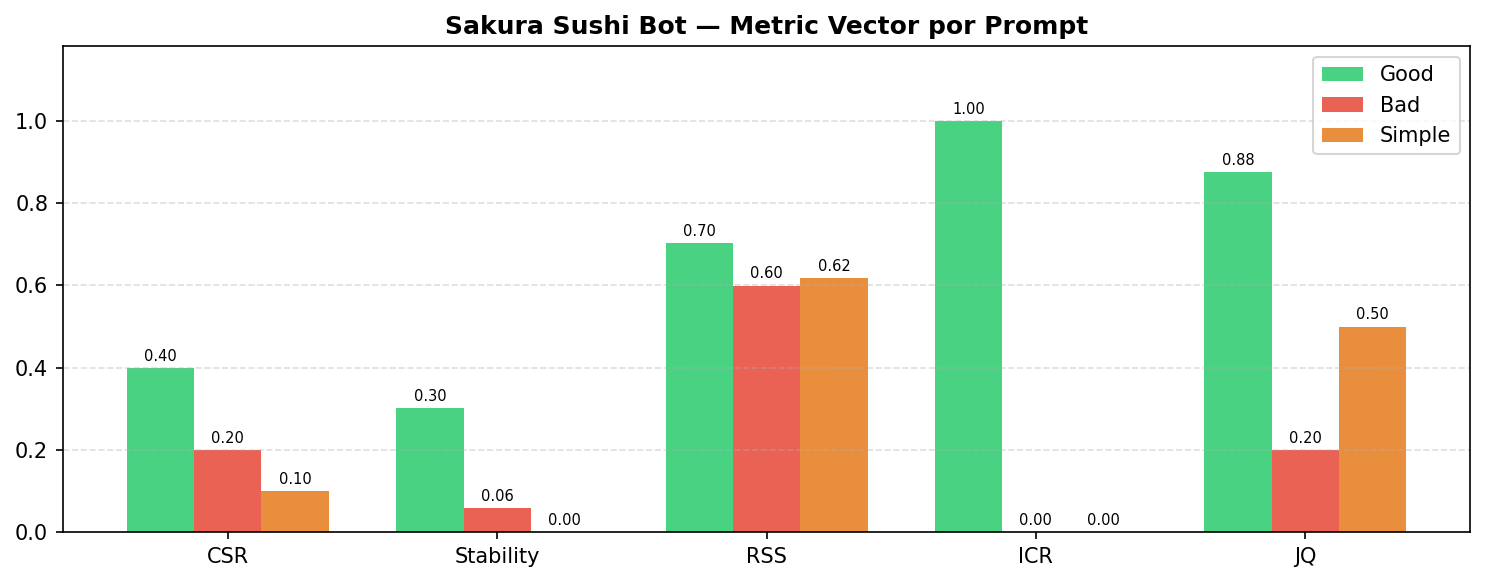
\includegraphics[width=0.72\textwidth]{figures/sushi_bar_overall.png}
\caption{Vector de métricas por variante de prompt ($K=10$, $\tau=0.90$, $T=0.7$). Cada grupo de barras corresponde a una señal; los colores indican calidad del prompt (verde = bueno, rojo = malo, naranja = simple).}
\label{fig:bar}
\end{figure}

\begin{figure}[h]
\centering
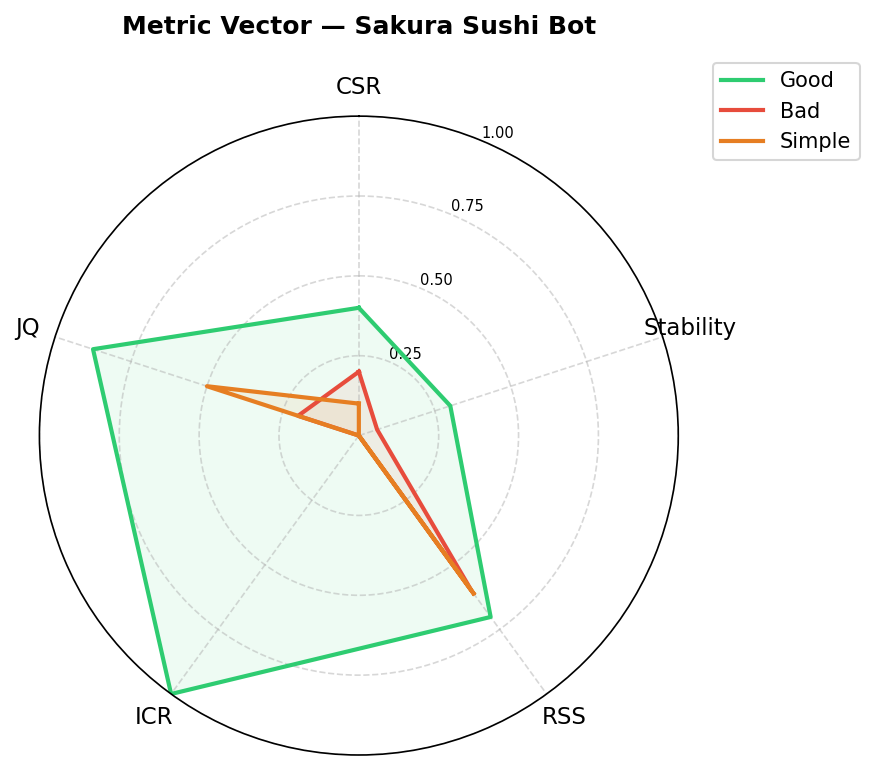
\includegraphics[width=0.48\textwidth]{figures/sushi_radar.png}
\caption{Gráfico de radar del vector completo de métricas por variante de prompt. El prompt bueno (verde) llena el polígono en las cinco señales; los prompts malo y simple muestran patrones de colapso distintos que revelan diferentes modos de fallo.}
\label{fig:radar}
\end{figure}

\subsection{Análisis}

\paragraph{CSR y Stability: las instrucciones comportamentales imponen comportamiento consistente.}
Las tres variantes están correctamente ordenadas: Bueno (CSR = 0.400, Stability = 0.301) $>$ Malo (0.200, 0.060) $>$ Simple (0.100, 0.000). Los valores absolutos de CSR son menores que en evaluaciones factuales típicas porque las consultas comportamentales son genuinamente multi-válidas en ausencia de instrucciones explícitas ---incluso un prompt bueno no puede eliminar completamente la variación semántica entre las $K$ muestras. El prompt simple alcanza Stability mínima ($= 0.000$): el modelo improvisa un enfoque comportamental diferente en casi cada muestra, produciendo entropía semántica máxima.

\paragraph{RSS solo no puede distinguir malo de simple.}
Puntajes RSS: Bueno = 0.702, Simple = 0.617, Malo = 0.599. El prompt bueno es correctamente identificado como el mejor por RSS, pero malo y simple son casi indistinguibles ---y su ordenamiento está invertido (simple $>$ malo). La explicación es que la similitud por embedding captura semántica a nivel de tema: una respuesta que intenta resolver una queja directamente y una que escala al manager ambas discuten el dominio de la queja y embedean de forma similar respecto a la referencia. RSS es insuficiente como discriminador único cuando los fallos del prompt consisten en seguir el protocolo incorrecto en lugar de salirse del tema.

\paragraph{ICR produce separación binaria perfecta.}
ICR cae de 1.000 (Bueno) a 0.000 para Malo y Simple ---separación binaria perfecta. El prompt bueno siempre invoca la palabra clave de escalado \textit{encargado} en los cinco tipos de consulta relevantes; el prompt malo instruye explícitamente contra el escalado y el prompt simple no provee ningún protocolo. Esto ilustra el valor de ICR como compuerta determinista: cuando una restricción está definida, su violación se detecta con certeza y sin varianza de juez.

\paragraph{JQ revela violación activa de protocolo en el prompt malo.}
El hallazgo multi-señal crítico es la brecha entre Malo (JQ = 0.200) y Simple (JQ = 0.500). RSS invierte este ordenamiento; JQ lo corrige. El prompt malo instruye activamente al modelo a violar el protocolo correcto ---ofrecer reembolsos directos por quejas, proveer remedios caseros para intoxicaciones alimentarias, confirmar reservas incompletas sin solicitar datos faltantes--- y el modelo sigue estas instrucciones incorrectas de forma consistente. El prompt simple, en cambio, produce respuestas improvisadas que a veces son aceptables para consultas directas, resultando en un JQ promedio mayor. Este es el patrón ``consistentemente incorrecto'' a nivel de protocolo: comportamiento consistente (CSR = 0.200) con respuestas que sistemáticamente contradicen el comportamiento objetivo, un fallo invisible para RSS pero expuesto por JQ.

\paragraph{Ninguna señal única es suficiente.}
La Tabla~\ref{tab:failures} resume los modos de fallo expuestos exclusivamente por cada señal.

\begin{table}[h]
\centering
\caption{Modos de fallo expuestos por cada señal en la evaluación comportamental.}
\label{tab:failures}
\begin{tabular}{lp{8.5cm}}
\toprule
Señal & Fallo que expone \\
\midrule
CSR / Stability & Inconsistencia comportamental: el prompt simple improvisa cada vez \\
RSS             & Deriva semántica respecto al comportamiento de referencia (bueno vs.\ otros); insuficiente para violación de protocolo \\
ICR             & Incumplimiento de restricciones: la palabra de escalado nunca aparece en malo ni simple \\
JQ              & Violación activa de protocolo en el prompt malo; invisible para RSS e ICR solos \\
\bottomrule
\end{tabular}
\end{table}

\noindent Ninguna señal en forma aislada ordena correctamente las tres variantes de prompt ni expone todos los modos de fallo. El vector compuesto de métricas es necesario para cobertura diagnóstica completa.

\subsection{Efecto de $\tau$ y $K$}
\label{sec:tau_k}

Realizamos un análisis de calibración para caracterizar la sensibilidad de CSR y Stability respecto al umbral $\tau$. Con $\tau = 0.80$ y $K = 10$, más del 90\% de las consultas produjeron $n_\mathrm{clusters} = 1$, saturando CSR en 1.0 para todas las variantes de prompt y eliminando el valor discriminativo. La causa raíz es que \texttt{all-MiniLM-L6-v2} ubica respuestas factualmente similares a similitud coseno superior a 0.80 independientemente de la variación superficial. Elevar $\tau$ a 0.90 restaura estructura de clústeres no trivial.

Un análisis secundario sobre la grilla $\tau \in \{0.80, 0.85, 0.90, 0.95\}$ y $T \in \{0.7, 0.9, 1.1\}$ (prompt fijo: comportamental bueno, $K = 5$) mostró que la temperatura tiene efecto limitado en CSR: el rango a lo largo de $T = 0.7$--$1.1$ para un $\tau$ fijo es a lo sumo $\pm 0.05$. La palanca de sensibilidad principal es $\tau$. Estos resultados justifican $\tau = 0.90$ como el valor predeterminado recomendado para embedders sentence-transformer en el rango de 22M--110M parámetros, y confirman que la métrica es robusta a la variación típica en la temperatura configurada por el usuario.

Una consideración de implementación adicional surge con los modelos de chain-of-thought: \texttt{qwen/qwen3-32b} emite bloques \texttt{<think>...</think>} antes de la respuesta real. Estos tokens de razonamiento, cuando se incluyen en el texto embedeado, hacen que cada respuesta sea semánticamente única ---colapsando CSR y Stability a sus valores mínimos independientemente de la consistencia comportamental real. Deshabilitar el modo de razonamiento (o eliminar los tokens de razonamiento antes de embedear) es necesario al evaluar modelos con output de chain-of-thought. Del mismo modo, cuando un campo \texttt{context} provee conocimiento de dominio accesible para ambas variantes de prompt bajo evaluación, la asimetría de información que el experimento está diseñado para testear queda eliminada; el conocimiento de dominio debe estar incorporado exclusivamente en el prompt bajo evaluación, no en un contexto compartido.

% ─────────────────────────────────────────────────────────────────────────────
\section{Discusión y Limitaciones}
\label{sec:discussion}
% ─────────────────────────────────────────────────────────────────────────────

\paragraph{Por qué un vector y no un escalar.}
Tres líneas independientes de evidencia apoyan devolver $\mathbf{m}$ como output primario. UniEval \citep{unieval2022} muestra que la evaluación humana de NLG es multidimensional y que un evaluador unificado debe diseñarse explícitamente alrededor de esas dimensiones. GLaPE \citep{glape2024} demuestra cuantitativamente que una señal única (SC) puede correlacionar pobremente con la precisión. ArmoRM \citep{armorm2024} argumenta formalmente que la escalarización lineal de peso fijo de múltiples objetivos es demasiado rígida, y que se requiere ponderación dependiente del contexto para que un escalar sea principiado.

\paragraph{Limitaciones.}
Los componentes de Tier 2 introducen dependencias (acceso a logprobs, modelo NLI, modelo de reward) que no están disponibles en todos los entornos de despliegue. ICR requiere que el prompt contenga restricciones programáticamente verificables, lo cual no es universalmente el caso. La calibración de $S$ requiere un conjunto de anotaciones humanas o etiquetas de referencia. RSS captura proximidad semántica a nivel de tema pero no puede detectar fallos a nivel de protocolo: las respuestas que siguen el protocolo incorrecto y las que improvisan libremente pueden embedear a distancias similares de la referencia, haciendo que RSS sea insuficiente para distinguirlas. Para evaluación comportamental, JQ es la señal primaria para detectar violación de protocolo.

\paragraph{Incorrección consistente.}
CSR y SE miden estabilidad distribucional, no corrección. Un prompt que lleva al modelo a producir consistentemente la misma respuesta incorrecta producirá CSR alto y SE bajo ---valores que indicarían un prompt ``bien definido''--- sin implicar que las respuestas sean factualmente correctas. Esta limitación es inherente a cualquier métrica libre de referencia y está documentada en \citet{glape2024}. Los usuarios que necesiten validar corrección además de estabilidad deben activar RSS (si hay respuestas de referencia disponibles) o JQ.

\paragraph{Extensiones futuras.}
Dos señales están definidas en el framework pero se dejan para trabajo futuro. \textbf{RM (Puntaje de Modelo de Reward)}: cuando se dispone de un modelo de reward entrenado con datos de preferencia humana, el puntaje $\mathrm{RM}(p, x) = \sigma\!\left(\frac{1}{K}\sum_k R(p, x, y_k)\right)$ proporciona una señal de calidad aprendida complementaria al juez basado en rúbrica; las variantes multi-objetivo \citep{armorm2024} devuelven un vector que puede escalarizarse dinámicamente, evitando la rigidez de peso fijo. \textbf{PP (Perplejidad del Prompt)}: los prompts con menor perplejidad tienden a producir mejor rendimiento en tareas \citep{promptperplexity2022}; el componente normalizado $1 - \mathrm{PP}_n$ entra en $\mathbf{m}$ con la misma convención de signo que las otras señales, pero requiere acceso a log-probabilidades de tokens, que no todos los proveedores exponen. Ambas señales se excluyen de la implementación actual por requisitos de infraestructura que quedan fuera del alcance de una biblioteca de evaluación de propósito general.

\paragraph{Elección de $K$ y su efecto en las estimaciones.}
La cantidad de muestras $K$ afecta directamente la confiabilidad de CSR y SE. La Tabla~\ref{tab:k} resume el comportamiento esperado según el rango de $K$.

\begin{table}[h]
\centering
\caption{Efecto de $K$ en la calidad de las estimaciones de CSR y SE.}
\label{tab:k}
\begin{tabular}{p{2cm} p{3.5cm} p{3.5cm} p{3.5cm}}
\toprule
Rango de $K$ & CSR & SE & Recomendación \\
\midrule
$K \leq 3$ &
Inestable. El modo puede cambiar con una sola muestra diferente. &
Inestable. Con pocos clústeres, la entropía no es representativa. &
No recomendado. Suficiente solo para verificaciones rápidas. \\
\addlinespace
$K = 5$--$10$ &
Estimación razonable para prompts con comportamiento claro. &
Estimación aceptable. Varianza de Monte Carlo moderada. &
Configuración predeterminada. Adecuada para la mayoría de casos de uso \citep{glape2024}. \\
\addlinespace
$K = 20$--$40$ &
Estimación estable. El modo converge con alta probabilidad. &
Estimación confiable. Varianza de Monte Carlo baja. &
Recomendado al comparar prompts similares o cuando se requiere alta precisión \citep{selfconsistency2023}. \\
\addlinespace
$K > 40$ &
Ganancia marginal mínima. &
Ganancia marginal mínima. &
El costo adicional raramente justifica la mejora en precisión. \\
\bottomrule
\end{tabular}
\end{table}

\noindent El efecto es más pronunciado en SE que en CSR: CSR solo necesita estabilizar el grupo mayoritario, mientras que SE requiere estimar la masa de \textit{todos} los clústeres, incluyendo los minoritarios. Por tanto, para prompts con comportamiento ambiguo ---donde se espera entropía alta--- se recomienda usar $K \geq 20$ para que los clústeres pequeños estén correctamente representados.

% ─────────────────────────────────────────────────────────────────────────────
\section{Conclusión}
% ─────────────────────────────────────────────────────────────────────────────

La contribución central de este trabajo es una descomposición principiada de la calidad del prompt en señales ortogonales y medibles de forma independiente. La descomposición importa porque los fallos de prompt son heterogéneos: inconsistencia, violación de protocolo, incumplimiento de restricciones y deriva semántica son fenómenos distintos que requieren detectores distintos. Colapsar todo en un único puntaje no agrega información --- la destruye.

La implicación práctica para los profesionales es que la elección de qué señales activar es en sí misma una decisión diagnóstica. Un prompt que puntúa bien en CSR pero mal en JQ es un tipo de fallo diferente al que puntúa mal en ambos --- el primero es consistentemente incorrecto, el segundo es incoherente. El vector hace visible esa distinción; un escalar no puede.

La limitación fundamental del núcleo obligatorio es que mide consistencia, no corrección. Esto no es una deficiencia a corregir sino un límite de alcance deliberado: la reproducibilidad requiere métricas libres de referencia, y las métricas libres de referencia no pueden verificar el ground truth. Los usuarios que necesitan garantías de corrección deben proveer respuestas de referencia (RSS), definir restricciones verificables (ICR), o aceptar el trade-off de reproducibilidad de un juez (JQ). El framework está diseñado para hacer ese trade-off explícito en lugar de ocultarlo dentro de un puntaje opaco.

% ─────────────────────────────────────────────────────────────────────────────
\bibliographystyle{plainnat}
\bibliography{refs}
% ─────────────────────────────────────────────────────────────────────────────

\end{document}
